\documentclass[../Main.tex]{subfiles}

\begin{document}

The preceding chapters of this document have meticulously delineated the architectural framework and the technological foundations employed in the system's development process. However, without distinct solutions and initiatives, the system might have remained indistinguishable within the extensive landscape of business solutions and unsuitable in other environments like Vietnam. This chapter aims to shed light on how the issues are identified in the development progress of the project and the personalized strategies and innovations that contributed to the system's uniqueness and enhanced its efficacy and relevance in a dynamic business environment.

\section{Display custom text}
\label{section:custom-font}
In the development process, the system encounters an issue when the user wants to display Vietnamese language texts and other special characters not in the ASCII character map. Vietnamese, with its complex diacritical marks and distinct character set, demands a high degree of precision in rendering, a task that is particularly challenging given the inherent limitations and operational mechanics of e-paper displays. This section will focus on how normal text is stored and processed in constrained environments like ESP32 and the problem of performance over resource usage. 

\subsection{UTF-8 vs. UTF-16}
\label{encoding}
UTF-8 and UTF-16 are both encoding formats used for representing text in computers, each with its unique handling of character sets, including special characters like those in the Vietnamese language. Unlike ASCII, where each character uses one byte to store, UTF-8 uses one to four bytes per character, making it highly capable of 1,112,064 valid character codes while still being backward-compatible with ASCII's old code. On the other hand, UTF-16 uses fixed-length two or four bytes per character, balancing the space efficiency of UTF-8 and the simplicity of fixed-length encoding. In the scope of this project, both encoding formats are compatible with processing Vietnamese characters to display on screen, each with its unique strengths and weaknesses. UTF-8, while enhancing the efficiency in memory and storage, still has drawbacks when parsing variable-length characters. The ESP32 must decode UTF-8 encoded strings into Unicode code points and then translate these into bitmaps. This process can lead to processing overhead and is more CPU-intensive compared to dealing with a fixed-length encoding like UTF-16.

\subsection{Two ways of process and display text}
\label{2-ways-process}
To be displayed properly on the screen, the text has to be converted to a bitmap image, stored in the form of an array of bytes. This process can be achieved by converting from an image of characters (Figure \ref{fig:thedotfactory}) or directly from the font file to corresponding byte arrays. The main goal of both two conversion ways is to create a mapping from every character to the corresponding bytes array, which is a step in the display process illustrated in Figure \ref{fig:font-display}. Due to the specific nature of frequently displaying Vietnamese characters, the project uses the second option, with the help of the TheDotFactory tool, to convert all the Vietnamese and Latin characters mapped to the byte arrays.
\begin{figure}[h]
    \centering
    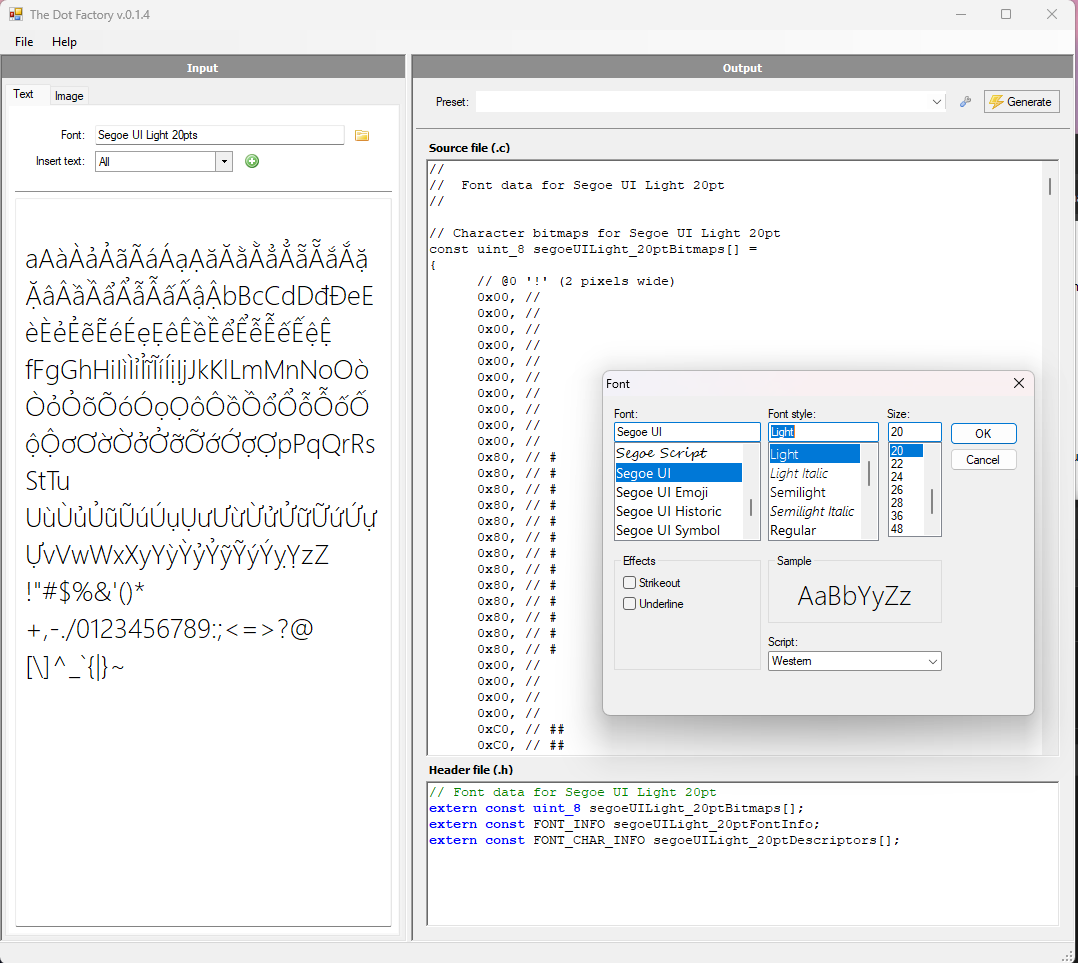
\includegraphics[width=0.8\linewidth]{doc/imgs/thedotfactory.png}
    \caption{UI of TheDotFactory tool}
    \label{fig:thedotfactory}
\end{figure}

\begin{figure}[H]
    \centering
    {\fontsize{10pt}{8pt}\selectfont 
        \begin{tikzpicture}[node distance=2.5cm, auto]
            \node (proc1) [process, minimum width=4cm, text width = 4cm, minimum height = 1.5cm] {\textbf{Iterate over string}\\\verb|“àăảBcd123@”|};
            \node (proc2) [process, below of=proc1, minimum width=4cm, text width = 4cm, minimum height = 1.5cm] {\textbf{Character}\\\verb|'à'|};
            \node (proc3) [process, right of=proc2, minimum width=4cm, text width = 4cm, minimum height = 1.5cm, xshift=3cm] {\textbf{Bytes-array lookup}\\"0x00 0xF2 0x21 ..."};
            \node (proc4) [process, right of=proc1, minimum height = 1.5cm, xshift=3cm] {\textbf{Display}};
            
            \draw [arrow] (proc1) -- (proc2);
            \draw [arrow] (proc2) -- (proc3);
            \draw [arrow] (proc3) -- (proc4);
            \draw [arrow] (proc4) -- (proc1);
        \end{tikzpicture}
    }
    \caption{Overall process of text displaying}
    \label{fig:font-display}
\end{figure}

In the text-processing task, looking for the bytes array of each character is the most resource-consuming task, especially in an extensive character set. In resource-limited systems like ESP32-C3 Supermini in the project, it is crucial to balance between saving as many resources as possible and processing data in a reasonable time. However, the way data is organized in the exported file from TheDotFactory does not effectively solve the problem of processing performance and resource conservation when having to store and process 228 different characters, including Latin letters, accented Vietnamese, special characters, and numbers. This issue, combined with the encoding formats discussed above, leads to two ways of storing and mapping from the character to its corresponding bytes array, with a big difference in performance and resource usage between the two.

\subsection{First Solution}
The first of the two solutions mentioned above is a practical and straightforward approach focusing on the flexibility and scalability of the character set. The mapped character set is stored in an array of multiple character map definitions, where each character is associated with a structure that contains its display properties (width) and the corresponding byte array for rendering (code structure below), making the retrieval of byte data for each character straightforward and intuitive. This method is particularly suited for systems where a direct and easy way to access the display data for each character is highly recommended, especially for a fixed and known set of characters.

{\fontsize{8pt}{8pt}\selectfont 
    \begin{verbatim}
  typedef struct 
  {
    char16_t * chr;                                     // index character, utf-16
    uint8_t width;                                      // dynamic width
    const char matrix[MAX_HEIGHT_FONT*MAX_WIDTH_FONT/8];// bytes-array (41*32/8)
  } FT_IDX;
  
  typedef struct
  {    
    const FT_IDX *table;
    uint16_t size;
    uint8_t Height;
  } cFONT;   // custom Font
    \end{verbatim}
}
The index character \verb|chr| defined in the struct above uses UTF-16 as the encoding format. Although it is not as memory-efficient as UTF-8 encoding format as discussed in section \ref{encoding}, UTF-16 encoding brings ease of character comparisons while UTF-8 requires checking multiple bytes for non-ASCII characters (above 126), which appear the most frequently in the Vietnamese language. The flow chart \ref{fig:flow-chart1} below shows the details of the process displaying a Vietnamese string on the screen.
\begin{figure}[H]
    \centering
    {\fontsize{9pt}{8pt}\selectfont 
        \begin{tikzpicture}[node distance=2.5cm, auto]
            \node (start) [startstop, minimum width=4cm, minimum height = 1.5cm, rounded corners=2.4em] {\textbf{UTF-8 String} \verb|“àăảBcd123@”|};
            \node (proc1) [process, below of=start, minimum width=4cm, text width = 4cm, minimum height = 1.5cm] {\textbf{Convert to UTF-16}\\\verb|u“àăảBcd123@”|};
            \node (proc2) [process, below of=proc1, minimum width=4cm, text width = 4cm, minimum height = 1.5cm] {\textbf{Iterate over string}\\\verb|u'à'|};
            \node (dec1) [decision, below of=proc2] {\textbf{End of string?}};
            \node (stop) [startstop, right of=dec1, xshift=2cm] {\textbf{Finish}};
            \node (proc3) [process, below of=dec1, minimum width=4cm, text width = 4cm] {\textbf{Search in character map}};
            \node (dec2) [decision, below of=proc3, text width = 1.8cm] {\textbf{Found index character?}};
            \node (proc4) [process, right of=dec2, xshift=2cm] {\textbf{Get bytes-array}};
            \node (proc5) [process, below of=proc4] {\textbf{Display}};
            
            \draw [arrow] (start) -- (proc1);
            \draw [arrow] (proc1) -- (proc2);
            \draw [arrow] (proc2) -- (dec1);
            \draw [arrow] (dec1) -- node[anchor=south] {Yes} (stop);
            \draw [arrow] (dec1) -- node[anchor=east] {No} (proc3);
            \draw [arrow] (proc3) -- (dec2);
            \draw [arrow] (dec2) -- node[anchor=south] {Yes} (proc4);
            \draw [arrow] (dec2.west) -- ++(-0.5,0) -- node[midway, left] {No} ++(0,2.5) -- (proc3.west);
            \draw [arrow] (proc4) -- (proc5);
            \draw [arrow] (proc5.west) -- ++(-6.2,0) -- ++(0,10) -- (proc2.west);
        \end{tikzpicture}
    }
    \caption{UTF-16 text handling process}
    \label{fig:flow-chart1}
\end{figure}

In terms of memory, this method stores a character set and occupies around 169 bytes per character map for 228 characters. For all 228 characters in the set, this method occupies a total of \(169 \times 228 = 38,532\) bytes or 37 kilobytes. This is also affected by the compiler padding and alignment, so this calculation provides an approximated number based on the struct layout of the character set. However, most bytes-arrays of each character in this project only take up around 40 bytes on average, which, in fact, only costs \(228 \times 40 = 9,120\) bytes, or 9 kilobytes of actual data, meaning there are still many redundant space unusable with this method. Also, the data of the processing task, which includes the converted UTF-16 string and other variables in the process, is not accounted for, making an even higher total memory occupation. Currently, this is not a big problem with ESP32-C3 Supermini, but when the system gets more complicated or is implemented in smaller microcontrollers, another approach is highly recommended to balance performance and resources.

\subsection{Second Solution}
The second solution uses the segment method combined with the lookup table, optimizing resource and time efficiency even more, especially in a constrained environment. In this method, each character is not directly mapped to its bytes-array but to the start index and the length of its array, and the array containing these character maps is a lookup table. In this way, the bytes array will be stored in one extensive single array, which reduces memory overhead significantly compared to the first straightforward method. Also, having a map that links each character to its corresponding byte range in the array allows for fast lookup and retrieval, making the rendering process more efficient, especially when dealing with larger sets of characters or more frequent character lookups, as would be the case when rendering text from strings.

However, finding the index character in the lookup table is also a time- and resource-consuming task as it usually iterates through the array to get the data corresponding to the character. Therefore, the lookup table is divided into three segments based on the use frequency, and each segment contains a group of characters that share mostly the same frequency range. This will boost the lookup time as it does not require iterating over a single array to find needed information. However, because Vietnamese characters in the UTF-8 table are distributed differently from the use frequency and the limited time of the project, the segments are still divided based on the UTF-8 table, with the first segment containing characters of ASCII table, the second segment containing the first half of Vietnamese character set, and the third segment containing the second half. To speed up the lookup process in each segment, the index character is converted to the corresponding Unicode point, and binary search is also used, which is implemented in \verb|binarySearchInSegment()| function in the code structure shown below.

{\fontsize{8pt}{8pt}\selectfont 
    \begin{verbatim}
  typedef struct 
  {
    int chr; // index character, Unicode point
    uint8_t width;  // dynamic width, used to determine the byte array's length
    int index;  // start index at byte map table
  } FT_MAP;

  typedef struct
  {    
    const FT_MAP *ASCII_table; // segmentSize = 95 characters from 32 to 126
    const FT_MAP *vn_table;    // segmentSize = 66 characters
    const FT_MAP *VN_table;    // segmentSize = 67 characters
    uint8_t Height;            //character's height, in pixels
  
    const FT_MAP * binarySearchInSegment(
      int unicodePoint, 
      const FT_MAP* segment, 
      size_t segmentSize
    );
    
    const char *table;
  } sFONT;   // custom Font with Segment Management
    \end{verbatim}
}

 The flow chart \ref{fig:flow-chart2} below shows the details of the process displaying a Vietnamese string on the screen in the second method.

\begin{figure}[H]
    \centering
    {\fontsize{7pt}{8pt}\selectfont 
        \begin{tikzpicture}[node distance=2cm, auto]
            \node (start) [startstop, minimum width=3cm, minimum height = 1.2cm, rounded corners=2.5em] {\textbf{UTF-8 String} \verb|“àăảBcd123@”|};
            \node (proc1) [process, below of=start, minimum width=1cm, text width = 4cm, minimum height = 1cm, yshift=0.5cm] {\textbf{Iterate over string}\\\verb|“à”|};
            \node (dec1) [decision, below of=proc1] {\textbf{End of string?}};
            \node (proc2) [process, below of=dec1, minimum width=2cm, text width = 4cm, minimum height = 1cm, yshift=-0.2cm] {\textbf{Convert to Unicode point}\\\verb|224|};
            \node (stop) [startstop, right of=proc2, xshift=2cm, rounded corners=2em] {\textbf{Finish}};
            \node (dec2) [decision, below of=proc2, text width = 2cm, minimum width=3cm, minimum height=1cm, yshift=-0.4cm] {\textbf{Compare to segment ranges}};
            \node (proc3) [process, below of=dec2, minimum width=4cm, text width = 7cm, minimum height = 2cm, yshift=-1.3cm] {\textbf{Binary search in corresponding segment}\\(Segment 1: Latin characters)\\(Segment 2: First-half Vietnamese characters)\\(Segment 3: Second-half Vietnamese characters)};
            \node (dec3) [decision, below of=proc3, text width = 1.8cm, yshift=-1cm] {\textbf{Found index character?}};
            \node (proc4) [process, below of=dec3, yshift=-0.6cm] {\textbf{Get bytes-array from bytes table}};
            \node (proc5) [process, below of=proc4] {\textbf{Display}};
            
            \draw [arrow] (start) -- (proc1);
            \draw [arrow] (proc1) -- (dec1);
            \draw [arrow] (dec1.east) -- node[anchor=south] {Yes} ++(2,0) -- (stop.north);
            \draw [arrow] (dec1) -- node[anchor=east] {No} (proc2);
            \draw [arrow] (proc2) -- (dec2);
            \draw [arrow] (dec2) -- node[anchor=east] {Found} (proc3);
            \draw [arrow] (dec2.east) -- node[anchor=south] {Not found} ++(2.5,0) -- (stop.south);
            \draw [arrow] (proc3) -- (dec3);
            \draw [arrow] (dec3.east) -- node[anchor=south] {Not found} ++(2.5,0)  -- ++(0,3) -- (proc3.east);
            \draw [arrow] (dec3) -- node[anchor=east] {Found} (proc4);
            \draw [arrow] (proc4) -- (proc5);
            \draw [arrow] (proc5.west) -- ++(-3,0) -- ++(0,17.5) -- (proc1.west);
        \end{tikzpicture}
    }
    \caption{UTF-8 text handling process}
    \label{fig:flow-chart2}
\end{figure}

In this solution, Unicode Point is used instead of the original UTF-8 encoding format, which performs better in character comparisons than UTF-8 and UTF-16. However, a function to convert from UTF-8 characters to Unicode points is still needed, and the lookup array in each segment is sorted in ascending order based on the Unicode points of its character elements for the binary search function. In terms of memory, each character map takes up around only 9 bytes, and the single bytes array occupies around 9000 bytes on average, making a total of \(9\times228+9000=11,052\) bytes, or 11 kilobytes, of the character set. Also, this calculation is estimated on the code structure, not taking the data during the process into account, and actual memory usage might slightly differ due to factors like alignment and padding specific to the compiler and the architecture.

Overall, the logic for accessing and using the data in this second solution becomes slightly more complex, requiring correctly handling the mapping and indexing into the byte array. However, this method leverages the advantages of both segmentation and binary search, effectively reducing the search space and improving lookup times, making it well-suited for handling a large set of characters efficiently on systems with limited resources like the ESP32.

\section{Solutions for managing devices}
Currently, this project handles and communicates to the \gls{EPD} devices via MQTT Broker, which requires a 2.4GHz Wi-Fi connection from the devices. This method is suitable in most cases when Wi-Fi infrastructures are widely available and easy to set up. There are also other ways of managing \gls{EPD} devices, and each method has its advantages and drawbacks. This section will comprehensively discuss each proposed solution to delineate their differences, providing a deeper understanding of their strengths and limitations. Additionally, the section will delve into the rationale behind selecting the Wi-Fi solution, offering insights into its suitability and effectiveness for the current project and the future plan to support a wide range of flexible management.

\subsection{Central Dock}
In the general system, a central component is required to act as a bridge between the server and the \gls{EPD} devices (figure \ref{fig:flow-chart3}). This component needs sufficient resources to handle large numbers of devices and process enormous amounts of data from the server. Also, depending on the \gls{EPD} devices, this central component will have specific features and functions.

\begin{figure}[H]
    \centering
    {\fontsize{7pt}{8pt}\selectfont 
        \begin{tikzpicture}[node distance=2cm, auto]
            \node (user) [process, minimum width=1cm, minimum height = 1cm] {Users};
            \node (server) [process, right of=user, yshift = 2cm, xshift = 1.5cm] {Server};
            \node (dock) [process, right of=server, yshift = -2cm, xshift = 1cm] {Central dock};
            \node (epd1) [process, right of=dock, yshift = 2cm, xshift = 2cm] {EPD device};
            \node (epd2) [process, below of=epd1] {EPD device};
            \node (epd3) [process, below of=epd2] {EPD device};
            
            \draw [arrow] (user) -- (server);
            \draw [arrow] (server) -- (user);
            \draw [arrow] (user) -- (dock);
            \draw [arrow] (dock) -- (user);
            \draw [arrow] (server) -- (dock);
            \draw [arrow] (dock) -- (server);
            \draw [arrow] (dock) -- (epd1);
            \draw [arrow] (dock) -- (epd2);
            \draw [arrow] (dock) -- (epd3);
        \end{tikzpicture}
    }
    \caption{General management system}
    \label{fig:flow-chart3}
\end{figure}

\subsection{Battery-less \gls{EPD} devices}
With its bi-stable nature that the display can hold an image for an extended period without any power supply, the \gls{EPD} device may not need a battery to function properly. It only consumes power when the display is being updated, and most of the energy used is from the ESP32 board. This advantage of e-paper display leads to a management solution for the use case when minimal power consumption is crucial, and a frequent data update is not essential. As such, the central component will have to handle the data update and display task of multiple individual \gls{EPD} devices, which is now only the display panel.

A Raspberry Pi board can meet these requirements to become a central dock of the system. With 48 GPIO pins equipped, this device can connect and transmit data to the \gls{EPD} devices via the SPI interface. Also, it is a powerful mini-computer capable of handling multiple tasks simultaneously and supports various programming languages, including Python, which is often used for \gls{EPD} programming due to its simplicity and vast library support. On top of that, Rasberry Pi is relatively small compared to other equivalent mini-computers, which brings enormous benefits to the system, which has limited space and needs mobilities. This setup also significantly reduces the cost of setting up the \gls{EPD} devices system, which is crucial in small businesses.

To display data, an \gls{EPD} device connects to the dock via GPIO pins, which also provide power for the display task. After the data is displayed, the \gls{EPD} device can disconnect from the dock, and the data remains displayed on the screen until a new display is needed. The \gls{EPD} panel can also connect to the dock via Near Field Communication (NFC), which can also transfer power wirelessly to the \gls{EPD} devices. This connection method can open great potential for managing \gls{EPD} devices when users can directly display data on devices right from their phones or any NFC-support devices. The diagram below shows the new device management flow, with the Rasberry Pi acting as the central dock to receive, handle, and transmit data to \gls{EPD} devices. The central dock can be a Rasberry Pi with the functions discussed above, or even users' phones and tablets if NFC is used as the connectivity between \gls{EPD} devices and the dock, and in that case, the users can directly control via the central dock without an intermediate server.

However, there are also drawbacks to this management method, making it only suitable for some minor use cases. First, this method is incapable of frequent updates and handling a lot of \gls{EPD} devices. Users can only update one \gls{EPD} device at a time, which will take a lot of time to update multiple \gls{EPD} devices. Also, \gls{EPD} devices need to connect to the dock in a short range, which limits the placement and scalability of the displays, especially in larger or more complex setups. In this centralized system, if the central dock encounters an issue or fails, all connected \gls{EPD} panels will be affected, and this is a significant drawback in critical applications where continuous operation is essential. This drawback also makes the development of the central dock more complex as it has to be stable, fault-tolerant, and effective in dealing with different display content for each panel.

These disadvantages of the central local dock make this solution only practical in small and simple use cases when the disadvantages do not significantly impact the overall functionality or efficiency of the system.

\subsection{Current solution}
The current solution is designed to handle \gls{EPD} devices that are ESP32-C3 Supermini boards connected with \gls{EPD} panels, allowing them to interact with the system individually. In this solution, the central dock does not need to process an extensive amount of data compared to the dock in the above method and only needs to relay data between the server and the \gls{EPD} devices. The \gls{EPD} devices can connect to this central dock at long-range distances by Bluetooth Low Energy (BLE) or Internet, maintaining the flexibility and scalability of the system. There can be two types of central dock in this system, depending on the connectivity used by \gls{EPD} devices. First, if the \gls{EPD} devices use BLE as connectivity, the central dock has to be a local device, receiving data from the server and transmitting it to the devices via BLE. This connectivity type is beneficial for \gls{EPD} devices with poor battery life and limited data size because its data rate is only 2Mbps, which is inefficient for complex image data. Secondly, if the \gls{EPD} devices use Wi-Fi, this central device can be an MQTT Broker, which receives data from the server and publishes it to the subscribed \gls{EPD} devices via MQTT protocol. This method is currently used because it can solve the overall problem of managing multiple devices in various business scenarios. However, this approach also comes at the cost of longevity for the \gls{EPD} devices as Wi-Fi connectivity consumes more power than BLE and does not support sleeping mode in ESP32, which is also discussed in section \ref{subsection:resource}.

\subsection{Optimization and future work}
\label{opt}
Although having some advantages and handling effectively in various scenarios, this management approach still exposes many downsides in the actual environment. Firstly, \gls{EPD} devices need a good and long-lasting battery, which can increase the thickness and affect the visual look of the devices. Secondly, it increases the setup and maintenance cost of the system as the devices are more complex and expensive to ensure quality and effectiveness. Thirdly, this solution is generally designed for most common cases, which limits the flexibility of the system. Section \ref{section:optimization} will provide more insights into the works conducted to optimize the \gls{EPD} devices' performance and improve battery life. Another solution is combining the advantages of the first solution into this, making it aligned with small environments while also suiting more complex needs of larger use cases. In this scenario, an additional central dock is implemented between the MQTT broker and the devices for BLE and NFC connectivity in more minor use cases and for some tasks that do not require an Internet connection. In larger use cases when an Internet connection is mandatory, the server will store a wish list of each device containing the data assigned to but not displayed on the device yet. With this solution, the \gls{EPD} device can sleep and reconnect to the broker to get and handle missed requests in a short period of time. If the devices need to sleep for an extended period, the intermediate central dock can also wake them via BLE, which still functions when the device is in sleep mode. However, in the scope of this project, this combined solution has not yet been implemented due to the complexity of the development process. The current solution is tested and can handle well in the ideal environment, achieving the goal of designing and building the prototype of the project and making it the base for further optimizations.

\section{ESP32 Optimization}
\label{section:optimization}
As discussed in chapter \ref{chapter:Experiment} and the section above, the \gls{EPD} device's performance is currently just sufficient in the prototype stage and requires further optimization in both resources and battery life. This section will provide more details of the optimizing process, including tracking and addressing the issues.

\subsection{Battery}
In normal working conditions with a continuous Wi-Fi connection, ESP32-C3 takes an average of \(324mA \times 3.3V = 1.0692W\) at peak, which is calculated roughly based on resources load and the mode's typical consumption defined in the datasheet\cite{espdatasheet}. The table \ref{fig:power-consumption} below indicates the power consumption of each component in the device in the ideal environment and working conditions (Room temperature, 3.3V supply, infrequent e-paper refresh, constant Wi-Fi, LED off, and MQTT connection).

\begin{table}[H]
    \newcolumntype{M}[1]{>{\centering\arraybackslash}m{#1}}
    \newcolumntype{L}[1]{>{\raggedright\arraybackslash}p{#1}}
    \renewcommand{\arraystretch}{3} % Adjust for row height
    \centering{}
    \fontsize{9pt}{8pt}\selectfont 
    \begin{tabular}{| m{3cm} | m{2cm} | m{8cm} |}
        \hline
        \textbf{Components} & \textbf{Active Mode}  & \textbf{Note}                                                             \\ \hline
        CPU Consumption     & 40mA (avg.)           & CPU run at max speed 160MHz with other peripherals enabled                \\ \hline
        RF Consumption      & 276mA	                & RF current consumption at peak in 802.11n mode                            \\ \hline
        ePaper Consumption 	& 8mA (avg.)            & Typical current consumption with rare refresh frequency (maximum 100mA)   \\ \hline
        Total               & 324mA                 & Total current consumption at peak, actual rate may vary                   \\ \hline
    \end{tabular}
    \caption{Power consumption of device}
    \label{fig:power-consumption}
\end{table}

The current only way to improve battery life and reduce the constraints of devices is by optimizing CPU and RF loads, which can be achieved by strategically managing processes in the device. In the future, implementing a more extensive battery without affecting the visual look significantly is also an excellent option to improve the battery life of the devices. The section below will focus on resource optimization, reducing CPU load, overhead, and memory wastes, which also contribute to battery improvement.

\subsection{Resources}
\label{subsection:resource}
Here are the details of program usage in the ESP32-C3 board reported by PlatformIO before optimization. This VS code plugin illustrated in figure \ref{fig:inspect} below also provides more insights about each component's size and allocation, which is helpful for indicating and addressing the issues.

\begin{table}[H]
    \newcolumntype{M}[1]{>{\centering\arraybackslash}m{#1}}
    \newcolumntype{L}[1]{>{\raggedright\arraybackslash}p{#1}}
    \renewcommand{\arraystretch}{3} % Adjust for row height
    \centering{}
    \fontsize{9pt}{8pt}\selectfont 
    \begin{tabular}{| m{3.5cm} | m{1.7cm} | m{8.5cm} |}
        \hline
        \textbf{Section}            & \textbf{Size (bytes)} & \textbf{Description}                                                                                           \\ \hline
        Text                        & 677,023               & Size of the compiled machine code, stored in the flash memory of the ESP32.                                    \\ \hline
        Data                        & 237,964               & Size of initialized global and static variables. Initially stored in flash memory and then copied to SRAM      \\ \hline
        BSS                         & 672,304               & Size of uninitialized global and static variables. Stored in SRAM and zero-initialized when the program starts \\ \hline
        Total Storage (Text + Data) & 914,987               & Total storage in flash memory (4MB total)                                                                      \\ \hline
        Total RAM (Data + BSS)      & 910,268               & Total RAM usage (365KB actual total)                                                                           \\ \hline
        Overall (Text + Data + BSS) & 1,587,291             & Total firmware size, helpful for OTA updates                                                                   \\ \hline
    \end{tabular}
    \caption{Code usage before optimization}
    \label{fig:code-usage1}
\end{table}

\begin{figure}[H]
    \centering
    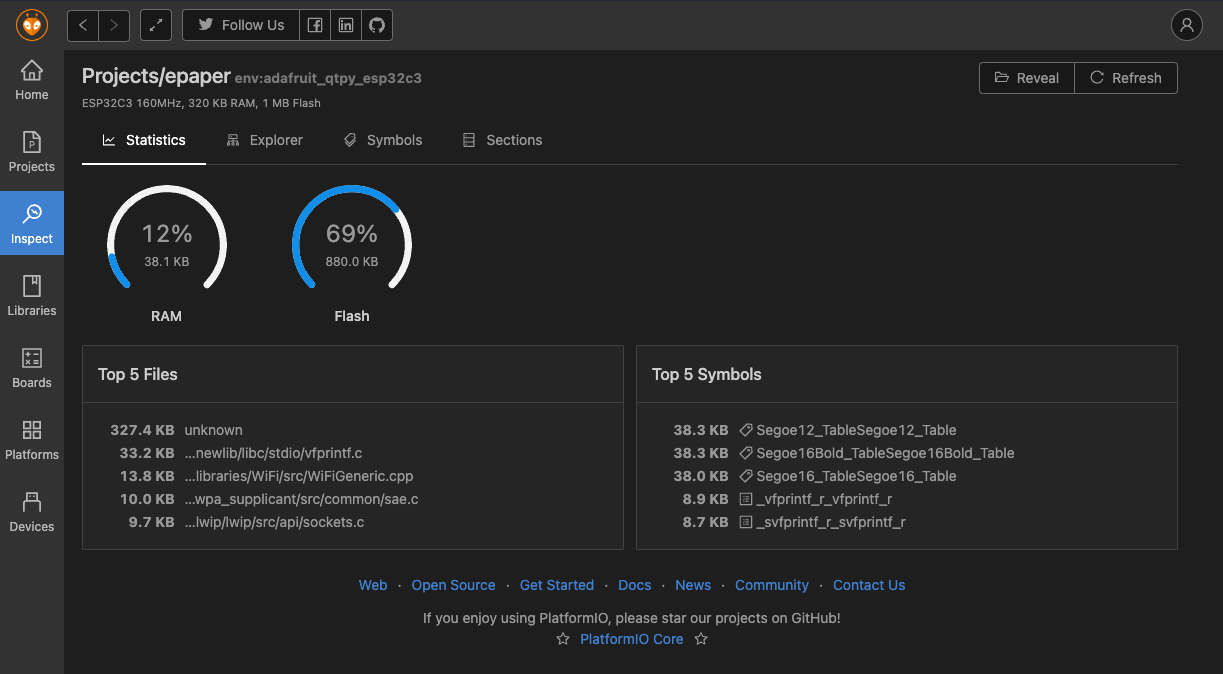
\includegraphics[width=0.8\linewidth]{doc//imgs/platformio-inspect.png}
    \caption{Inspect result of PlatformIO plugin}
    \label{fig:inspect}
\end{figure}

From the details provided in the table \ref{fig:code-usage1}, it is clear that exceeding 910KB of total RAM usage may lead to potential overhead and memory leaks and put constraints on the device if not properly managed and allocated. This also poses a risk of malfunctioning and battery draining, which decreases the overall performance of the devices a lot. To reduce Data and BSS usage and address this problem, one of the good practices is reducing the number of global and static variables if redundant and using dynamic allocation. Reducing tasks in the device also helps reduce the burden on CPU load, which can decrease CPU clock speed and thus improve battery life.

With the help of PlatformIO Inspect tools, a detailed analysis of the variables in the program has been conducted, revealing valuable insights into their size and sections. Moreover, ESP's useful libraries in resource management also help track resource usage at specific parts, providing a comprehensive picture of code structure (illustrated in figure \ref{fig:platformio-debug}). This detailed breakdown helps pinpoint particular areas where memory usage can be optimized. Thus, numerous issues have been effectively identified and addressed, making memory management efficient and improving overall application performance.

\begin{figure}[H]
    \centering
    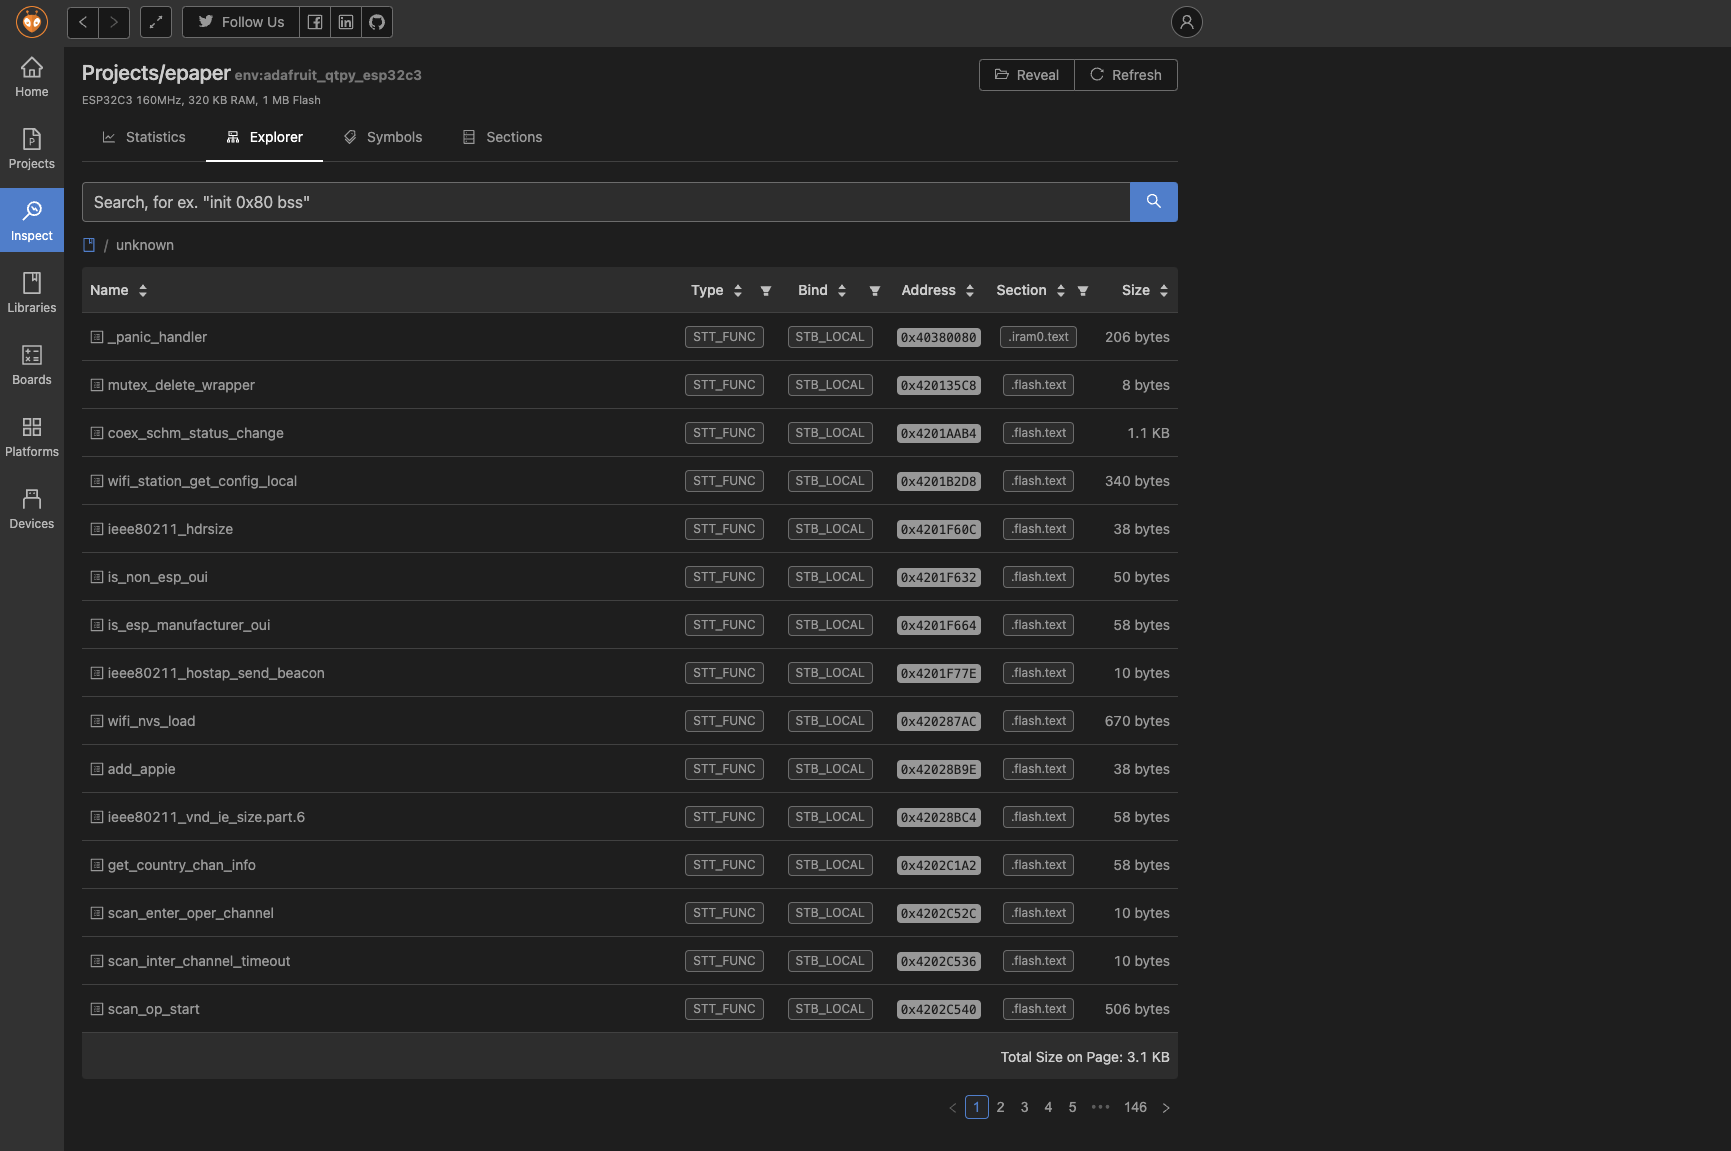
\includegraphics[width=0.95\linewidth]{doc//imgs/platformio-debug.png}
    \caption{Details about usage of each components in the code}
    \label{fig:platformio-debug}
\end{figure}

The most significant memory optimization work is changing the way of storing and processing custom Vietnamese text fonts, which is discussed in section \ref{section:custom-font}. The occupied size of an average font decreased three times to just 11KB, which overall reduces memory usage and lookup time, leading to reduced CPU and RAM load. A lot of duplicate, large, and unused variables are also identified, removed, and reallocated dynamically in numerous parts of the code. As a result, the code structure is well-optimized, saving resources while still ensuring the performance of the devices. The table \ref{fig:table_new-reports} below shows the memory usage after optimization.

\begin{table}[H]
    \newcolumntype{M}[1]{>{\centering\arraybackslash}m{#1}}
    \newcolumntype{L}[1]{>{\raggedright\arraybackslash}p{#1}}
    \renewcommand{\arraystretch}{3} % Adjust for row height
    \centering{}
    \fontsize{9pt}{8pt}\selectfont 
    \begin{tabular}{| m{4cm} | m{3cm} | m{3cm} |}
        \hline
        \textbf{Section}            & \textbf{Old size (bytes)} & \textbf{Size changed (bytes}  \\ \hline
        Text                        & 692,494                   & +15,471                       \\ \hline
        Data                        & 198,283                   & -39,681                       \\ \hline
        BSS                         & 420,482                   & -251,822                      \\ \hline
        Total Storage (Text + Data) & 890,777                   & -24,210                       \\ \hline
        Total RAM (Data + BSS)      & 618,765                   & -291,503                      \\ \hline
        Overall (Text + Data + BSS) & 1,320,259                 & -267,032                      \\ \hline
    \end{tabular}
    \caption{Code usage after optimization}
    \label{fig:table_new-reports}
\end{table}

In the actual environment, the frequency of data updates is not high, meaning most of the time, the \gls{EPD} device keeps the connection to the MQTT Broker and waits for new requests, which is a time-, resource-, and battery-wasting task. A periodical sleep mode can be implemented to address this problem; however, it will also deactivate the RF component in ESP32, which is responsible for the Wi-Fi connection\cite{esptechnical}. Although it can reconnect to Wi-Fi and the MQTT broker after a period of sleeping time, the device still has chances of missing requests from users, and if not configured to handle, this may lead to a lost information scenario, which is crucial in businesses. Another solution to this is also discussed in the previous section \ref{section:optimization}, which is currently not implemented yet. Other than that, the optimized system has been proven to handle tasks effectively in various testing conditions.

\section{Security and vulnerabilities}
A secure and reliable connection is paramount in a system that includes many devices communicating with each other and storing sensitive data. This project, however, had to go through a system hack that resulted in all users' data being deleted and sold on the black market. This experience, together with other security issues in the development process, has brought an urgency to enhance the system's security.
\subsection{MongoDB Hack}
Currently, MongoDB in the system is configured securely with the user's credentials and is being proxied behind a secure connection. However, on the first days of the development, with rudimentary configurations and exposing many vulnerabilities, the MongoDB server is "open" to the public with little protection from the system firewall. Several hacks targeting the MongoDB databases via the open port 27017 of the MongoDB server have been conducted by a hacker who deleted all collections and overwrote them with a recovery message (figure \ref{fig:atlas-hack}). The figure \ref{fig:mongo-pig} shows the messages from the hacker, demanding a payment of 0.025 BTC (equivalent to \$1,000) to recover the data; otherwise, the data will be "published on the darknet forums on the TOR network".
\begin{figure}[H]
    \centering
    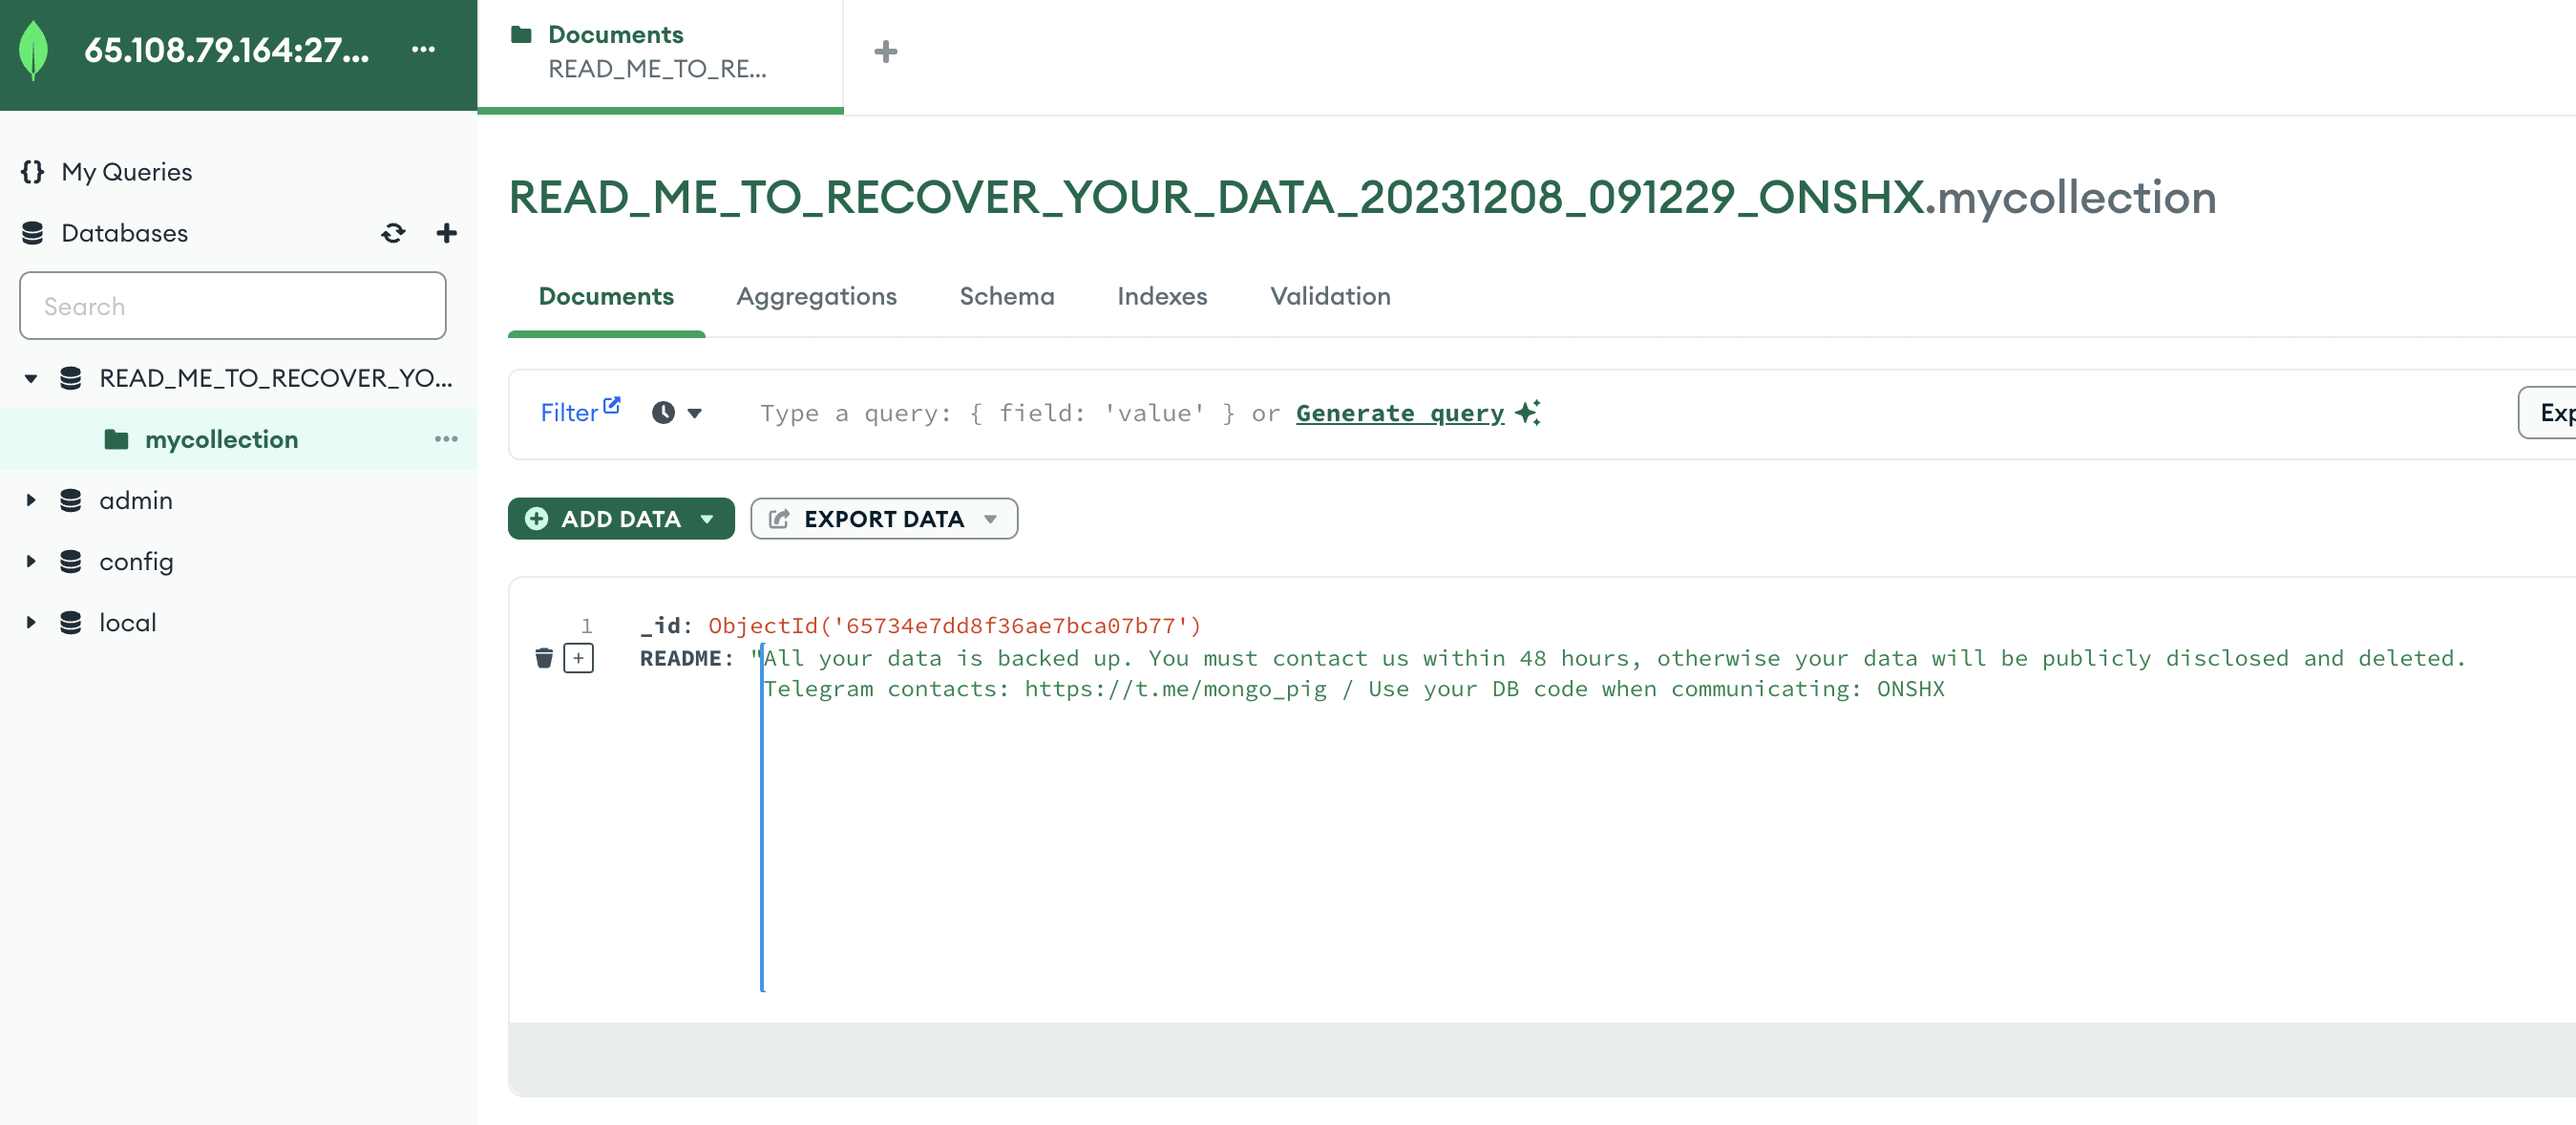
\includegraphics[width=0.9\linewidth]{doc/imgs/mongo-hack.png}
    \caption{Mongo Atlas dashboard showing the corrupted data}
    \label{fig:atlas-hack}
\end{figure}
\begin{figure}[H]
    \centering
    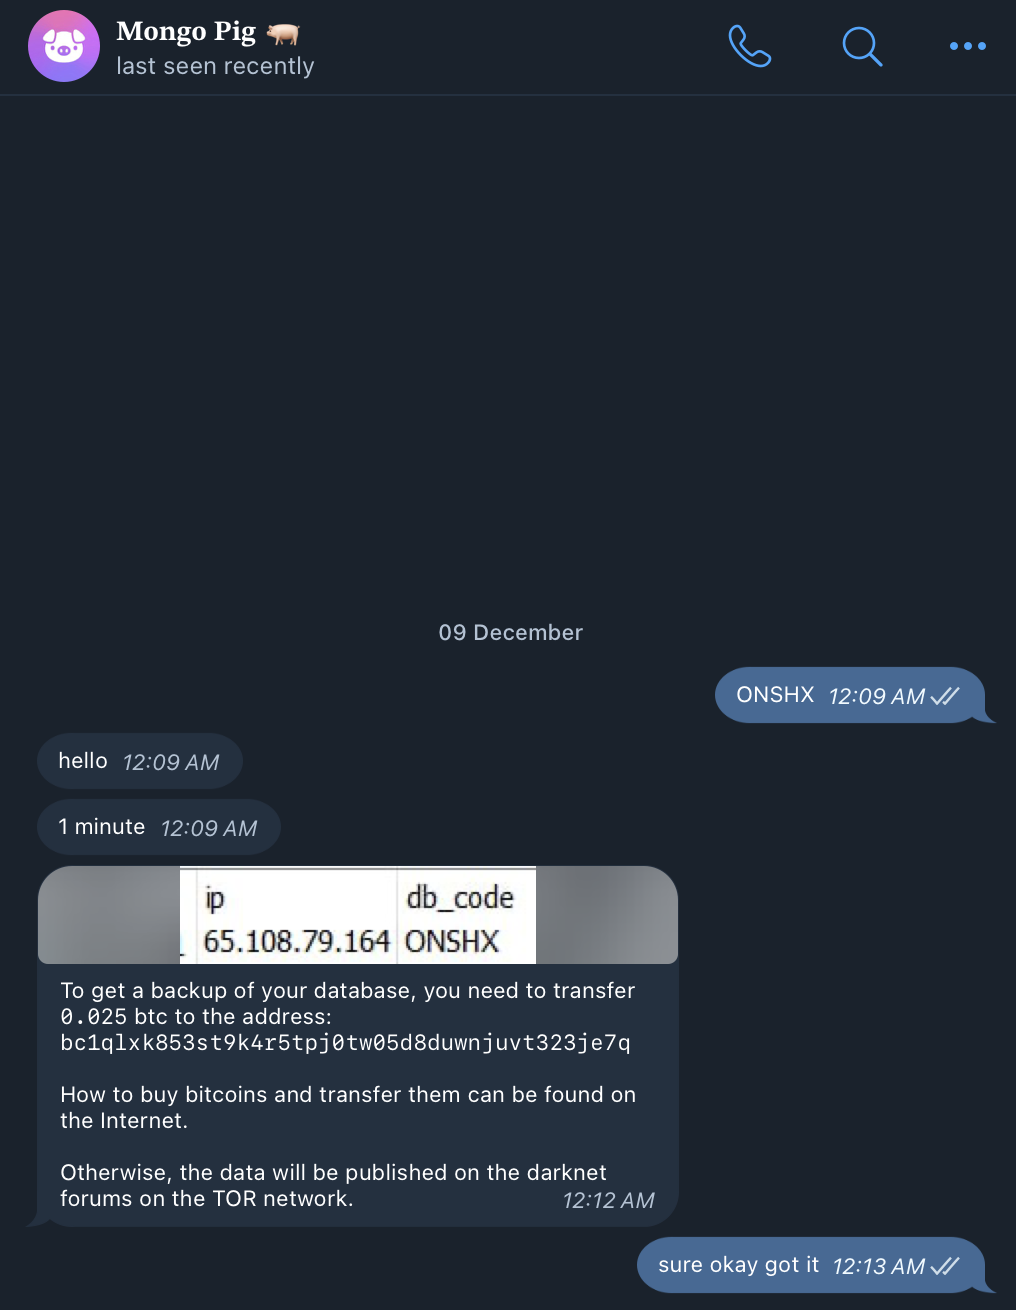
\includegraphics[width=0.5\linewidth]{doc/imgs/mongo-pig.png}
    \caption{Messages from the hacker}
    \label{fig:mongo-pig}
\end{figure}
 
\subsection{TLS/SSL and Certificate Authorities (CA)}
MongoDB is one of several tools used in the system that have open connections to other services, together with RabbitMQ and the web servers. Each tool comes with built-in mechanisms to protect data and communications and a logging system to trace down any abnormalities in the system. One of the critical features for enhancing security in both these systems is the implementation of TLS/SSL (Transport Layer Security/Secure Sockets Layer) protocols, using internal Certificate Authorities (CAs) to issue and verify digital server and client certificates.

In the internal CA, Root CA serves as the highest level of trust within the system's certificate hierarchy. It is responsible for self-signing its certificate and issuing Intermediate CA certificates. These Intermediate CAs bridge the gap between the Root CA and lower-level certificates. They inherit trust from the Root CA and are used to issue, verify, and revoke server and client certificates. In the services participating in the system, including MongoDB server, RabbitMQ broker, API server, and \gls{EPD} devices, server and client certificates are used to secure communication. Server certificates are used to encrypt data transmitted to and from servers, ensuring confidentiality. Client certificates authenticate users or devices, confirming their identity before granting access to specific resources or services. Also, the web server uses Cloudflare SSL certificates to implement secure HTTPS protocol between the user and the system. The image \ref{fig:certs} below illustrates the CA system used in the project. Certificate configurations and documentation are detailed inside the \verb|/certificates| folder in the project's GitHub repository.

\begin{figure}[H]
    \centering
    {\fontsize{7pt}{8pt}\selectfont 
        \begin{tikzpicture}[node distance=2cm, auto]
            \node (rootCA) [
                process, 
                minimum width=1cm, 
                text width = 4cm, 
                minimum height = 1cm
            ] {\textbf{Root CA}};
            \node (interCAs) [
                process, 
                below of=rootCA, 
                yshift=-1.2cm, 
                minimum width=8cm, 
                minimum height=2cm, 
                fill=none, 
                align=center, 
                on background layer, 
                text width=6cm
            ] {\ \ \\\ \ \\\ \ \\\ \ \\Intermediate CAs};
            \node (interCA1) [process, below of=rootCA, minimum width=2cm, minimum height = 1cm, yshift=-1cm, xshift=-2cm] {\textbf{Intermediate CA}};
            \node (interCA2) [process, right of=interCA1, minimum width=2cm, minimum height = 1cm, xshift=2cm] {\textbf{Intermediate CA}};
            \node (mongoCRT) [process, left of=interCA1, xshift=-2cm, yshift=1cm] {\textbf{MongoDB}\\Server Certificate};
            \node (rabbitCRT) [process, below of=mongoCRT] {\textbf{RabbitMQ}\\ Server Certificate};
            \node (web) [process, right of=interCA2, text width = 1.8cm, xshift=2cm, yshift=1cm] {\textbf{API Server}\\Client Certificate};
            \node (epd) [process, below of=web] {\textbf{EPD Devices}\\Client Certificate};
            
            \draw [arrow] (rootCA.west) -- ++(-1,0) -- ++(0,1) -- ++(3.1,0) node[midway, above] {Self signed} --(rootCA.north);
            \draw [arrow] (rootCA) -- (interCA1);
            \draw [arrow] (rootCA) -- (interCA2);
            \draw [arrow] (mongoCRT) -- (interCAs);
            \draw [arrow] (rabbitCRT) -- (interCAs);
            \draw [arrow] (web) -- (interCAs);
            \draw [arrow] (epd) -- (interCAs);
        \end{tikzpicture}
    }
    \caption{Certificates system}
    \label{fig:certs}
\end{figure}

By implementing this Internal CA infrastructure, the system can enable secure TLS/SSL connections between services, ensuring a robust and organized approach to digital security, safeguarding sensitive data, and maintaining the trust and integrity of online interactions.
\end{document}